\chapter{Solution design}\label{chapter:soldesign}


\section{Overview of the SPM tool}\label{section:ovv-spm}


\begin{figure}
	\centering
		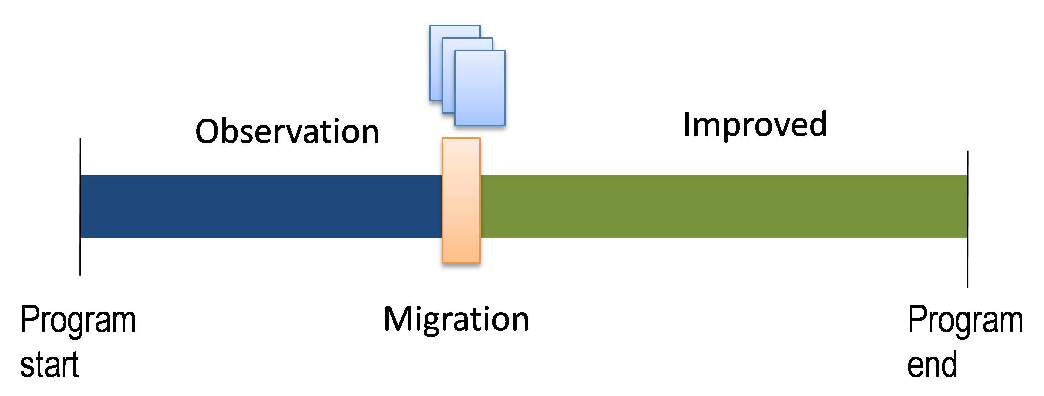
\includegraphics[width=.6\textwidth]{figures/spm-principle.eps}
		\caption[sampling-process]{TODO add caption}
		\label{fig:dstrategy}
\end{figure}

Figure [X] shows the high level operation of the SPM tool through time, which has three parts: the measuring part, the page migration and the improved part. The measuring part SPM measures the memory behavior of the guest process, where the length of this process is determined by the user and set in the overall SPM configuration. The page migration will reallocate the home of the pages according to the information obtained in the measurement phase and a pre-established policy. The length of the page migration phase depends solely on how long it takes to migrate the pages marked for this process. At the end, the improved phase lasts until the end of program execution, where it will again analyze the memory behavior of the program and print information at the end so that an analysis can be derived to find out whether there was an improvement on the performance after making the page migration.



\section{Strategy and alternatives of development}\label{section:strat}
In order to implement the desired functionality the idea is to adapt the code from one of the already working tools that access the PMU to the needs of the project. Two options were considered: perf and Intel numaTop, with the latter being chosen. It is worth noting that for the communication with the Performance Measurement Unit both tools make use of the same set of calls. A short description of both alternatives will be given in this chapter.

Figure [x] shows the overall working principle of the developed tool. The developed tool invokes the configuration capabilities from the kernel side, which then configures the physical PMU. Once configured and started the PMU starts passing samples to the kernel side, which passes them on to the measurement tool once the buffers are read. Upon a read in user space the sample will be passed to the custom tool for processing the samples. The control part will be in charge of coordinating the execution of all the parts of the program.

\begin{figure}
	\centering
		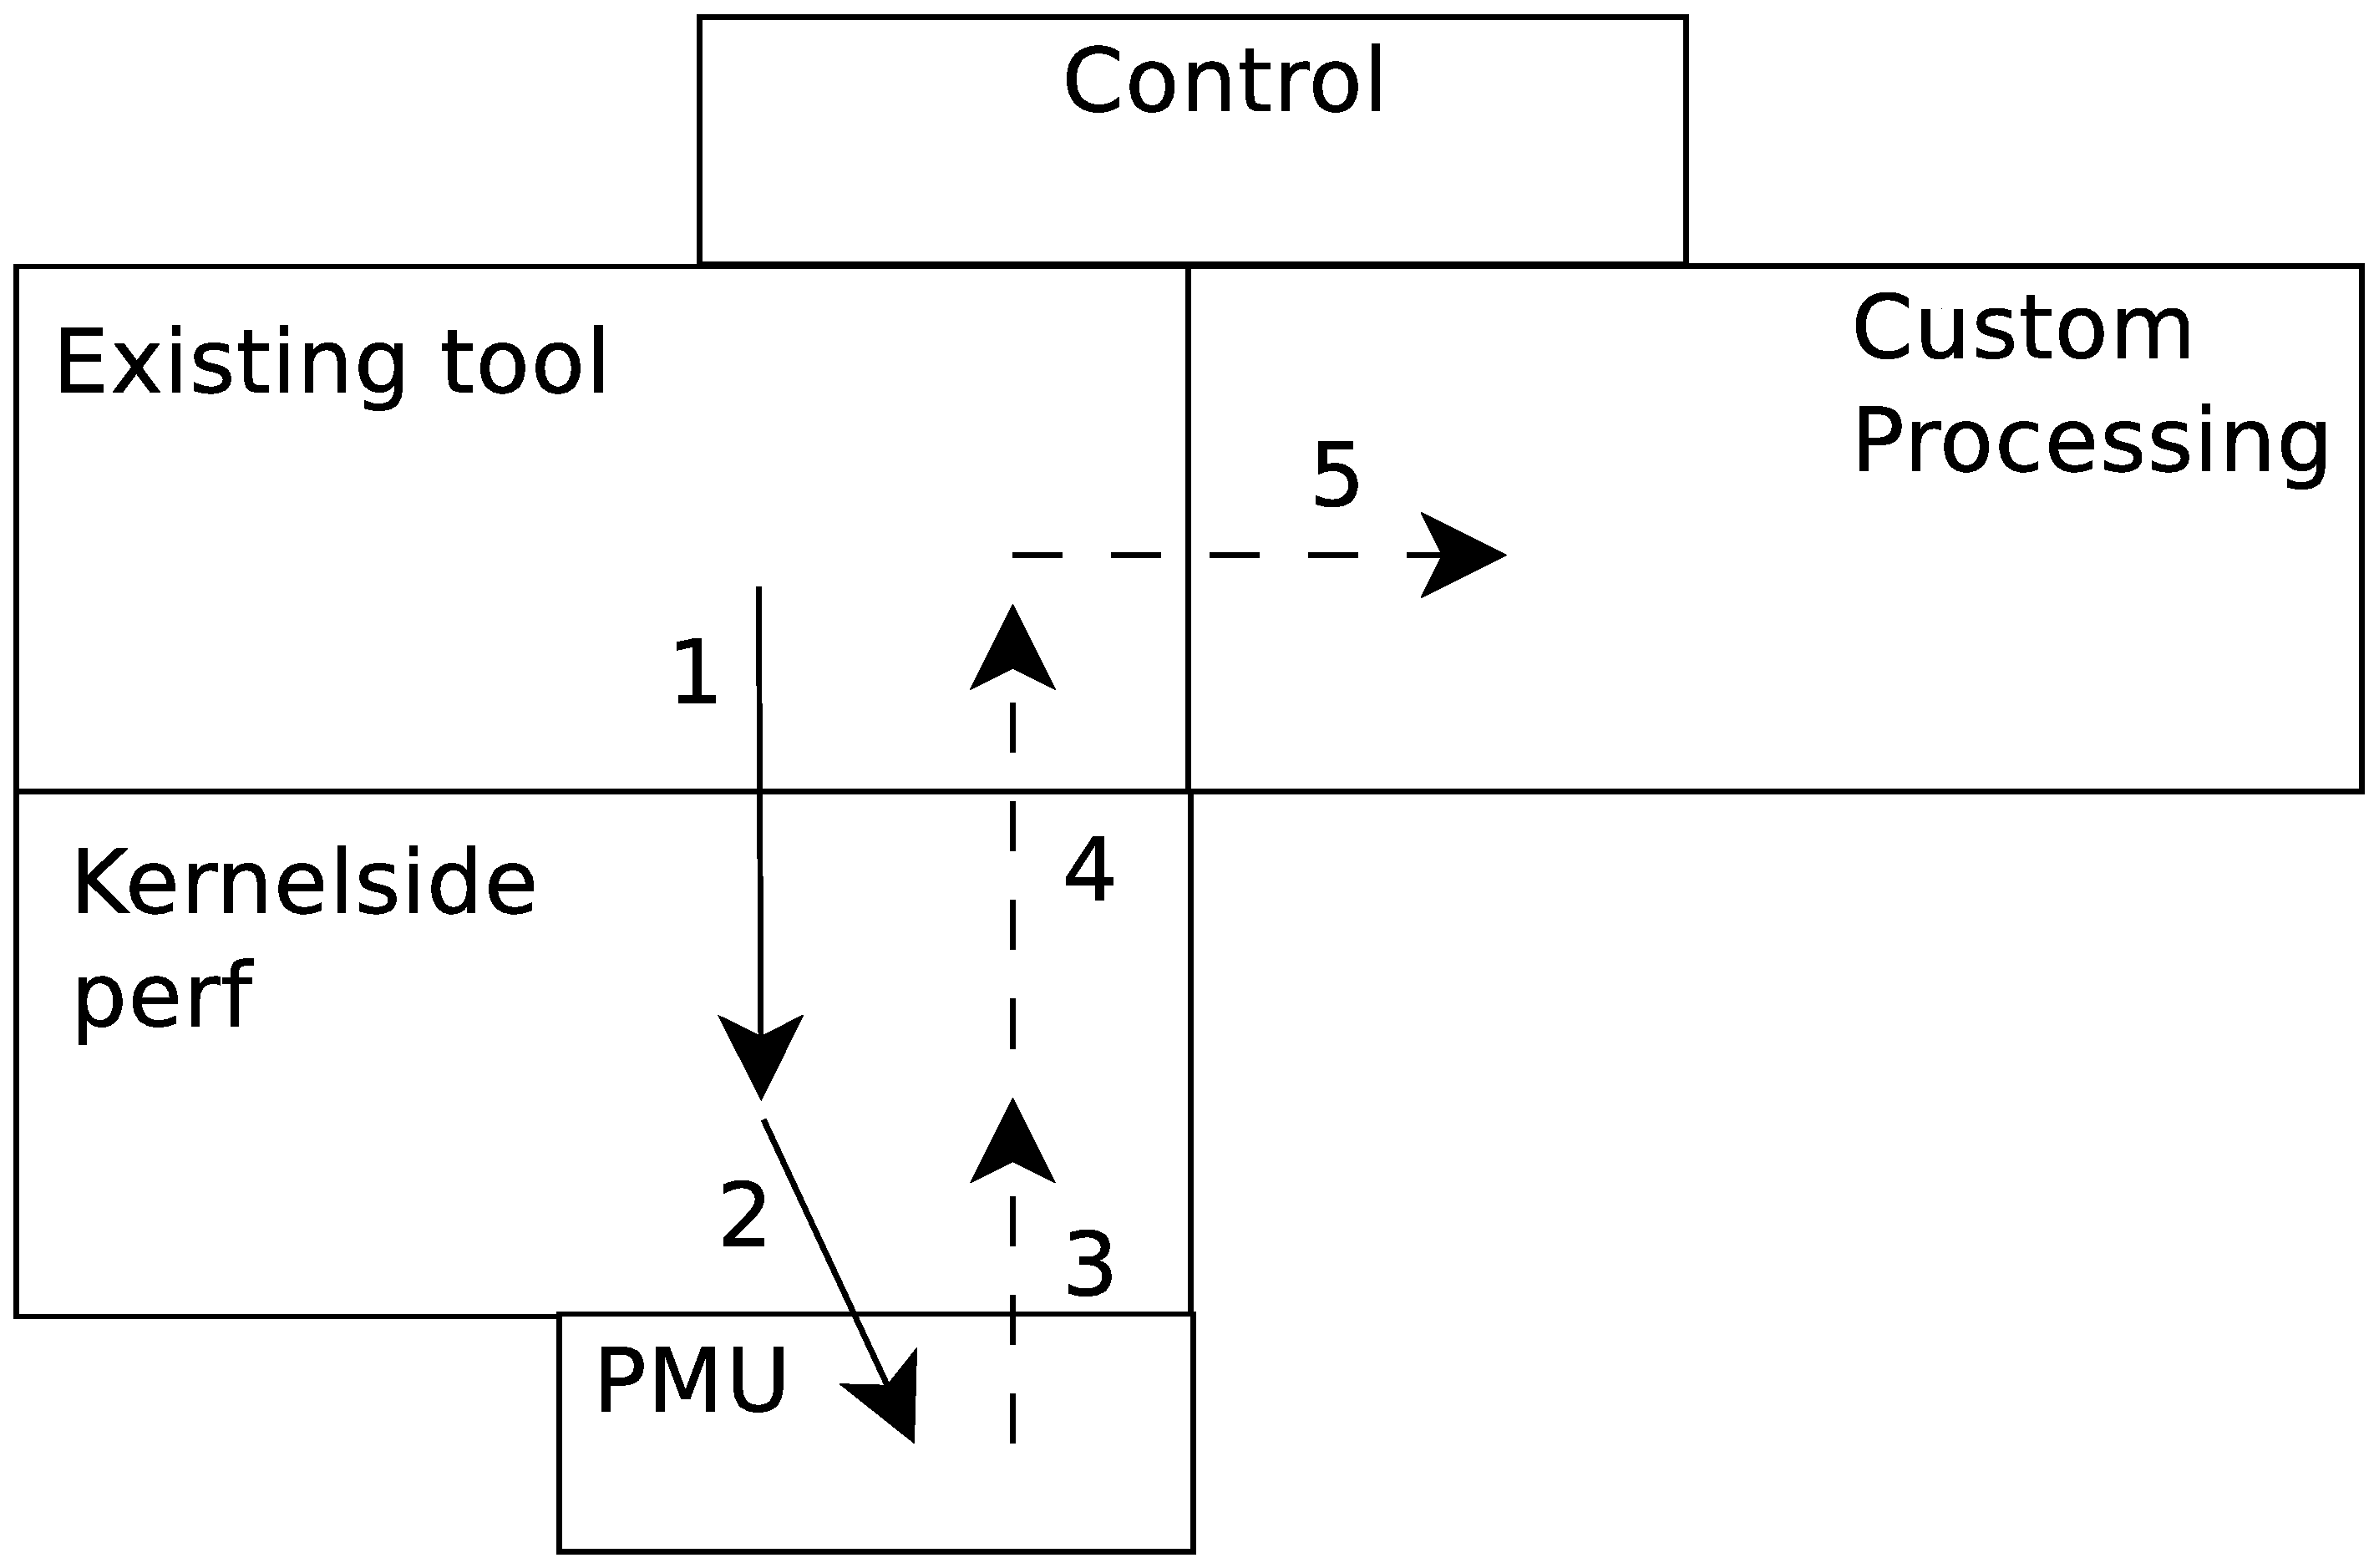
\includegraphics[width=.8\textwidth]{figures/dev-strategy.eps}
		\caption[basic-uma]{TODO add caption}
		\label{fig:dstrategy}
\end{figure}
\subsection{Perf user tools}\label{section:perf-ut}

This is the most comprehensive in terms of supporting events and covering a diverse range of architectures and performance events. Unfortunately this complexity together with the lack of documentation make the adaptation process a time consuming task and the end solution comprises a great number of source files, which cannot be shrunk without undertaking a large effort. 

The perf user tool \texttt{perf top} was adapted in order to have a constant and never ending access to the samples. In the function perf\_event process samples in the file builtin\_top.c a call is made to intercept the produced sample and analyzed according to our needs. The GUI of the executable is disabled.

\subsection{NumaTop}\label{section:numatop}
NumaTop provides a reduced functionality in comparison with the user side of perf, but it still provides all the functionality that is needed for this project. Its smaller code size helps to understand how the sample acquisition process works. The needed methods were grouped into a smaller file in order to make the number of source files smaller and around this the SPM code was built


\subsection{Evaluation}\label{section:sol-evltn}
NumaTop provides a reduced functionality in comparison with the user side of perf, but it still provides all the functionality that is needed for this project. Its smaller code size helps to understand how the sample acquisition process works. The needed methods were grouped into a smaller file in order to make the number of source files smaller and around this the SPM code was built.

\section{Communicating with perf's kernel side}\label{section:ovv-perfks}

\begin{figure}
	\centering
		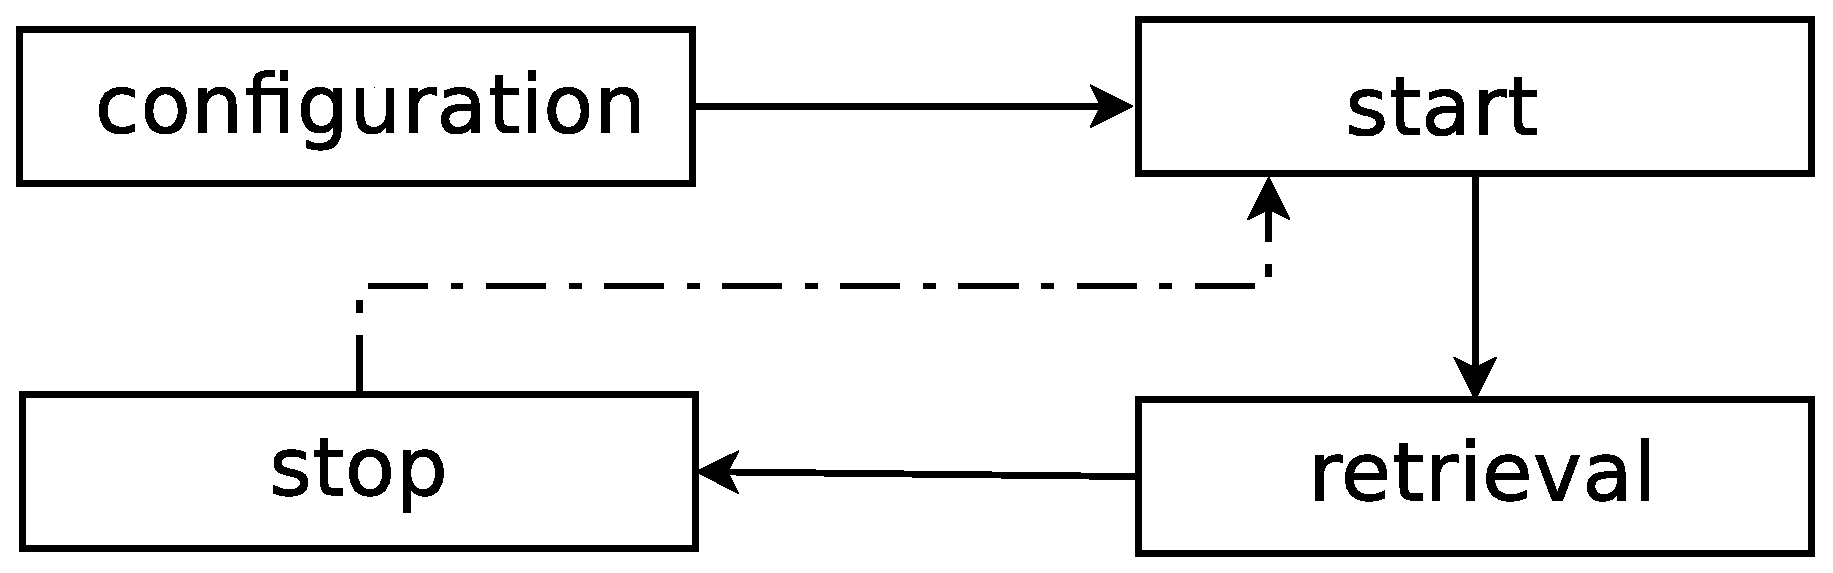
\includegraphics[width=.7\textwidth]{figures/sampling-process.eps}
		\caption[sampling-process]{TODO add caption}
		\label{fig:dstrategy}
\end{figure}

In order to be able to retrieve samples from the kernel side, a small amount of system calls have to be made, this section describes the flow for using the measuring system and lists the system calls used. Figure [x] shows an overview of the sampling process with its four stages: configuration, start, retrieval and stop.

\subsection{Configuration}\label{section:confgtn}
The configuration of the PMU is made for every event and for every CPU  that we want to watch. By making the system call with identifier \_\_NR\_perf\_event\_open. An actual call would take the form: 

\texttt{syscall(\_\_NR\_perf\_event\_open, attr, pid, cpu, group\_fd, flags) }

\begin{itemize}
	\item Attr: A struct of type perf\_event\_attr which specifies the sampling parameters, its fields are better explained in section [INSERT REF]. 
	\item Pid: Takes the value -1, in order to be able to monitor all the executing PID.
	\item CPU: Takes the identifier of the core whose PMU to configure.
	\item Group\_fd: For this implementation takes the value -1.
	\item Flags: For this implementation it takes the value 0.
\end{itemize}

After setting up the PMU the function mmap is called in order to create a file descriptor which will be used to read the samples. In order to create the descriptor, the first parameter of the mmap function call is NULL. The most important parameter in the PMU set up is the attr field because it specifies what we want to measure and how we want it.  

\subsection{Start and stop of the sampling}\label{section:start-sto}

To start and stop the sample unit the following system call is made: 
\\
\begin{center}
\texttt{ioctl(descriptor, constant, 0))}
\end{center}
Where descriptor is the file descriptor assigned to every combination of CPU and event and constant takes the value PERF\_EVENT\_IOC\_DISABLE or PERF\_EVENT\_IOC\_ENABLE depending on the objective.


\subsection{Retrieval and the reading the samples}\label{section:retr-reaf}

The file descriptor must be read periodically in order to collect samples. Given that the acquisition of the samples is made through low level I/O, the read is made by reading a chunk of certain number of bytes and it is up to the programmer to turn this stream into a suitable representation. 

The read of the descriptor is made using the mmap function, which takes as parameter the descriptor, the length of the read and the buffer where the read information will be kept.

\section{Important data structures}\label{section:important structs}

\subsection{The perf\_event\_attr struct}\label{section:pea-stru}

The perf\_event\_attr is the struct used to configure the PMU as shown in section [missing section]. In its fields the configuration parameters of a PMU are set. As it have a relative number of fields only the most important will be explained here. For the complete description of this struct it is advisable to check the man pages of the sys\_perf\_event\_open call and the document design.txt located on the root of the perf user side source three. This struct is defined in the kernel header perf\_event.h 
\begin{itemize}
	\item record\_type: For the use in our program will always take the value 4 (PERF\_TYPE\_RAW) since we are retrieving data from the hardware PMU. It is possible to collect data from other sources, such as the kernel itself, for instance.
	\item sample\_period: Specifies the number of instructions between consecutive samples. It is also possible to specify a frequency instead of a period by setting the use\_freq field.
	\item Precise\_ip: It is used to specify that the event to be read uses precise sampling(see section xx) 
	\item Config and config1: Config specifies the event to read as it is formed by concatenating the umask and the id. Config1 is used to specify any
 additional information that the event measurement requires. 
	\item Sample\_type: This field consists of the logic of the fields specified in the perf\_event\_sample\_format enumeration and determines which information is returned in every sample , for example PERF\_SAMPLE\_IP | PERF\_SAMPLE\_TID | and so forth.
	\item Disabled: Determines whether the sampling requires further additional activation.
\end{itemize}
     
\subsection{A perf sample}\label{section:pf-samplu}
     
The samples are retrieved from a sequential read to a file, so it is up to the programmer to give sense to this incoming information. The first information coming from a sample is the header, which follows the layout of the struct   perf\_event\_header. From this header we obtain two important pieces of information: the first one is the size of the sample, and the other is the type of the sample. For the type of the sample and our purposes it is only important the samples of type PERF\_RECORD\_SAMPLE. Once read the header, the next size bytes will belong to a sample. 

The information coming in a sample is determined by what was configured in the Sample\_type field when configuring the sampling. What is still unknown is the order in which the fields are returned. In order to figure this out it is better to refer to an existing implementation. For the consumption of the sample body the idea is to read each field and displace the reading position the number of bytes that a field occupies. The methods profiling\_sample\_read and ll\_sample\_read provide the sample reads to be used in the development. 
    
\subsection{The numatop core}\label{section:numatop-core}
The SPM tool is based on an adaptation of the numaTop methods used for communicating with the perf kernel side. This functions are located in the sampling-core.c file of the SPM sources, or on the numaTop sources themselves. 

The functions follow the logic stated in section (Coming with perfs kernel side) and they exist in two varieties, the methods with "profiling" in their name refer to the access of the registers that refer to a sampling value, such as the access to the offcore registers and the methods with "ll" refer to the load latency records, which are precise methods. Their functionality is very similar. 
\begin{itemize}
	\item The functions responsible for setting up the PMU are pf\_profiling\_setup and cpu\_ll\_setup
	\item The functions responsible for starting the PMU are pf\_profiling\_start and pf\_ll\_start 
	\item The functions responsible for stopping the PMU are pf\_profiling\_stop and pf\_ll\_stop
\end{itemize}
  
\section{Main layout of the spm tool }\label{section:ovv-perfks}

\begin{figure}
	\centering
		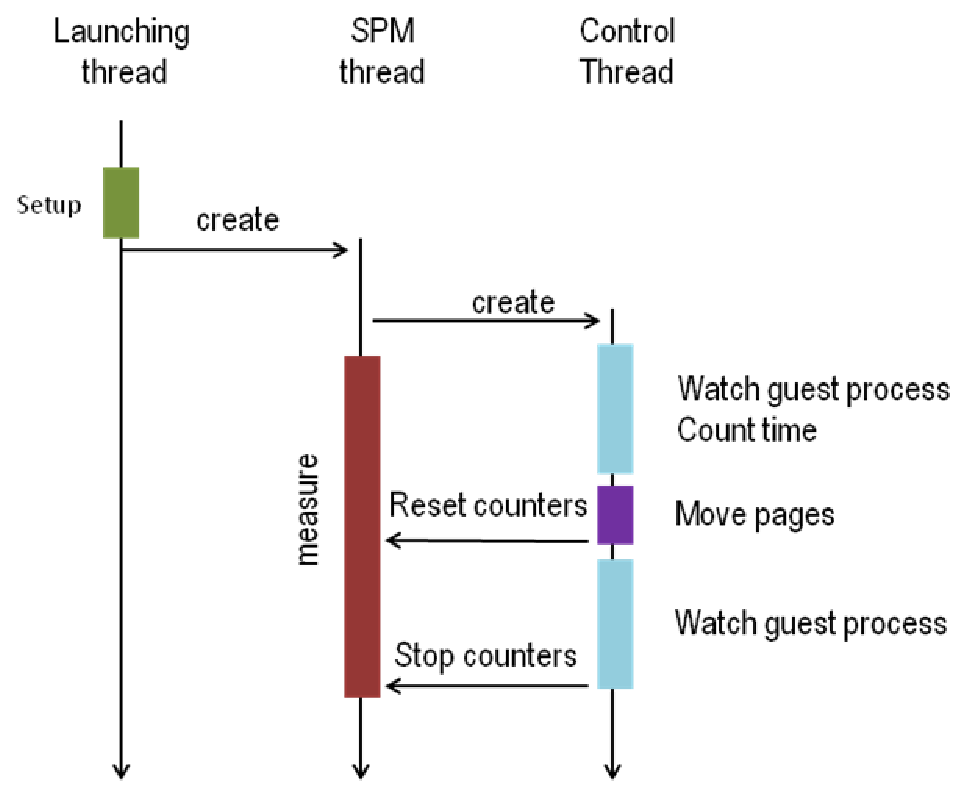
\includegraphics[width=.9\textwidth]{figures/sequence.eps}
		\caption[basic-uma]{TODO add caption}
		\label{fig:dstrategy}
\end{figure}

Figure [x] shows the overall principle of implementation of the SPM tool. The launching thread sets up the system and creates the SPM thread, which is in charge of collecting the samples from the numaTop core. The SPM thread then will launch the control thread, which controls the overall execution of the three phases, prints the statistics, invokes the migration and ensures that the observed process is executing on the background.

\section{Integration with Autopin+}\label{section:apin+intgr}

The SPM functionality is integrated into the code base of autopin+. For this purpose SPM’s sources are added to the ccmake configuration script (CMakeLists.txt).
For the calling of the SPM functionality within autopin+, a few additions to the autopin+ code are done:

\begin{enumerate}
	\item A new descendant of the PerformanceMonitor is created, which is then named PageMigrate.
	\item The recognition of the new class is enabled by adding the corresponding logic in the selection if present in the createPerformanceMonitors located in the Watchdog class.
	\item A new field is added to the PerformanceMonitor class together with the setter method, which allows it to retain the identifier of the process to watch. This is necessary because until now a performance monitor is enabled using the identifier of a thread and in the SPM tool the pid is employed to enable the tool.
	\item The start method is modified in order to invoke the init\_spm function. Before the invocation the configuration struct is created and the necessary fields are filled.
\end{enumerate}
	%Important structs for using the perf events system
	%perf_event_attr
	%evsel
	%The format of a perf sample
	%The numaTop sampling core (Explain how a sample is taken)
	%Page migration process explained
	%Phase I: Sample consumption and data gathering
	%Page migration
	%Phase II: PostMigration
	%Integration to Autopin+